
\documentclass{article}% use option titlepage to get the title on a page of its own.

\linespread{1.4}

\usepackage{lmodern}
\usepackage{listings}
\usepackage{color}

\definecolor{dkgreen}{rgb}{0,0.6,0}
\definecolor{gray}{rgb}{0.5,0.5,0.5}
\definecolor{mauve}{rgb}{0.58,0,0.82}

\usepackage{graphicx}
\graphicspath{ {./images/} }



\title{%
  Non-negative LASSO \\
  \large A Portfolio replication application}

\date{2019, February}
\author{Giovanni Misseri, Andrea Della Vecchia \\ \\ 
Business Economics and Finantial Data}
\begin{document}
\maketitle
\tableofcontents
\newpage
\section{Introduction}

Portfolio management has always been one of the most used way investors start approaching to financial investments. An important task in finance is indeed optimizing the revenue with respect to the risk of investing in a portfolio.

Markowitz in the '50, stated that single minded pursuit of high returns results in a poor strategy and rational investors need to balance their desire for high returns with low risk. So investing in a portfolio seems reasonable, indeed it diversify our investment and if we are able to spot profitable companies on which invest, we are guaranteed good revenue taking relatively low risk.
\\

There are mainly two strategies in portfolio management, active and passive managements. Active management tries to exploit the fluctuations of the market to gain as much as possible. On the other hand, passive management, tries to mimic the performance of an index. As one can easily notice, with active approach it's possible to loose great amount of money even investing on, on average, growing companies. On the other hand if we are able to well mimic a, on average, growing index, with passive approach we are guaranteed positive revenue.

Empirically is often the case passive approach outperforms active approach, also due to the transaction costs. In this work will try to propose two different solution to pursue respectively the passive and the active approach.

\newpage
\section{Shrinkage Methods}

If we have a feature or some measurements of an interesting phenomenon, is often the case that, given some related variables, we try to explain the phenomenon as a function of the related variables. The use of linear model, in case of linear relation between phenomenon and variables, is a good choice for two reasons: it gives good prediction and on the other hand, given the linear relation, it's highly interpretable. 

In general the more correlated variables we have, the "better" the model will be; but sometimes the presence of too much independent variables conditions the prediction error and also the presence of an high number of predictors limits the interpretability of the model. For these reasons one could decide to add a regularization term to its minimum least square problem.

\[
\min_{\beta_0 , \beta} \frac{1}{N} \sum_{i=1}^N (y_i-\beta_0 - \sum_{j=1}^p x_{ij}\beta_j)^2 + \lambda\sum_{j=1}^p |\beta_j |^q 
\]

Where $|\beta|^p$ is the $p$-norm of $\beta$.
\\

If in the regularized minimization problem we choose norm-two we obtain the ridge regression, if we choose the norm-one we obtain LASSO regression. 


It's easy to prove that shrinkage methods also solve an other type of problem related to ordinary least square. With OLS indeed the solution of the minimization problem is $ \beta_{ols}=(X^TX)^{-1}X^Ty$, decomposing $X$ through SVD, $X=V\Sigma U^T$, we get $\beta_{ols}=U\Sigma^{-1}V^Ty$. From this we can easily see that if $\Sigma$ is not invertible $\beta_{ols}$ could not be found.
\\

Shrinkage methods deal with this problem. Ridge regression ends up giving $\beta_{ridge}=U(\Sigma^2+\lambda I)^{-1} \Sigma V^T y$. Lasso regression's beta cannot be written in an explicit form, but the non-invertibility problem is solved due to the fact that, fixed $\lambda$, at the optimum, some beta will be equal to zero. Intuitively this is due to the feasible solutions space shape; indeed LASSO regression can be written as the following minimization problem.
\begin{equation}
 \min_{\beta} \sum_{i=1}^N ( y_i -\beta_0 -\sum_{j=1}^p x_{ij} \beta_j)^2 ~~subject~to~\sum_{j=1}^p |\beta_j| \leq t
\end{equation}

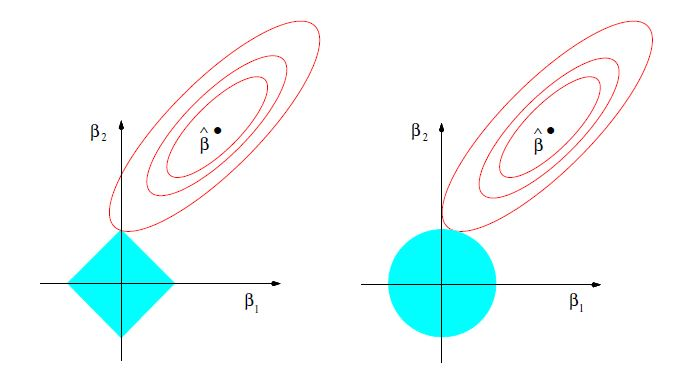
\includegraphics[scale=0.75]{lasso}

\subsection{LASSO and Portfolio Replication}

A replicating portfolio for a given asset or series of cash flows is a portfolio of assets with the same properties. So the principal problem of building a good replicating portfolio for a certain financial aggregate index is finding the right components of the index, the one able to represent the index itself. 

With the problem posed like that, the link between lasso regression and portfolio replication it's evident. Indeed one interesting properties of lasso regression is the variable selection consistency, so using lasso regression we are guaranteed, under certain condition, that it will select an optimal subset of variables in order to explain our dependent variable. It's clear now that lasso could help on the selection of the subset of time series that will be part of the portfolio; so we will select a subset of an index' components  able to explain the index itself.
\\

Here comes one problem, how to use lasso, a cross-sectional regression method, on a dynamic dataset? We will use a moving window approach, so we will assume that the data inside a window of fixed length are time invariant, and we compute lasso on that.

Another problem is the interpretation of the resulting model. Ones we find the solution to the lasso minimization problem, we have the beta related to all the variables, in our case the components of the index. Some beta will be equal to zero, so they will be excluded by our portfolio, for all the other beta a nice interpretation is available. 

If we carefully think to lasso as it has been defined in $(1)$, we approximate an index, the used one will be $Sp500$, as a function of some of it's components, conditioning to the fact that the sum of the associated beta is less than a given $t$. Practically we will work on the daily log-returns, and so our response and regressors will be all daily log-return; said that it's easy to see that $t$ can be seen as the initial budget and each beta is the volume of the "suggested" investment in a certain asset. Later on we will exploit this fact to run simulations using the different proposed methods.

For an active approach everything works fine, a positive beta will be an investment and a negative beta will be a short sell. On the other hand, for passive approach, it could be forbidden or in general doesn't make much sense to use short sell. For this reason to our estimates we need to add the constrain of non-negativity.
\\

Considering that also elastic net regression has the consistency variable selection, we will try to select the assets both with lasso and elastic net regression. Some comparison will be done on that.

\subsection{Dataset Analysis}
The major problem dealing with this kind of financial data is the high variability of the index from one day to another. In our case, this means that the behaviour of  $Sp500$ at time $t+1$ is very difficult to predict at time $t$.
\begin{figure}[h!]
  \centering
  \includegraphics[scale=0.6]{daily_var.png}
  \caption{Daily values of $Sp500$ index}
  \label{daily_var}
\end{figure}

We start our analysis with the simpler case in which we want to replicate $Sp500$ at time $t$ knowing the values of the $500$ assets (our $x$ variables) composing the index. Since there will be some correlation between the assets we can ask ourselves how many of them are really needed. Keeping the number of variables low is not only useful for having a less complex model but also, if we want really to invest in the assets and reproduce the index, to avoid the payment of a large number of fees (one for each purchase). On the other hand, the more we simplify the model ignoring some variables, the more our replication of the index will result to be inaccurate. With Lasso we can control the number of variables different from $0$ adjusting the value of the regularization parameter $\lambda$, we show the results below: 

\begin{figure}[h!]
  \centering
  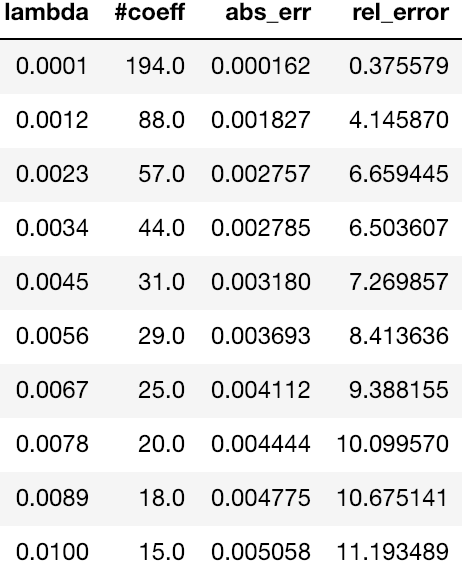
\includegraphics[scale=0.6]{err_lambda.png}
  \caption{$Sp500$ replication varying $\lambda$}
  \label{err_alpha}
\end{figure}

Unfortunately, this is not very useful. At time $t$ we are interested in predicting $Sp500$ at time $t+1$ and according to that planning our financial strategy. The simplest way to do it is by using our linear model shifting $y_t$ by a step $h$ with respect to $x_t$:
\begin{equation}
 \min_{\beta} \sum_{t=1}^T ( y_{t+h} -\beta_0 -\sum_{j=1}^p x_{tj} \beta_j)^2 ~~subject~to~\sum_{j=1}^p |\beta_j| \leq C.
\end{equation}

As mentioned before, due to the high variance of the process this naive approach is quite inefficient and this will be a problem in the following sections where we will try to build up a financial strategy based on these predictions

\begin{figure}[h!]
  \centering
  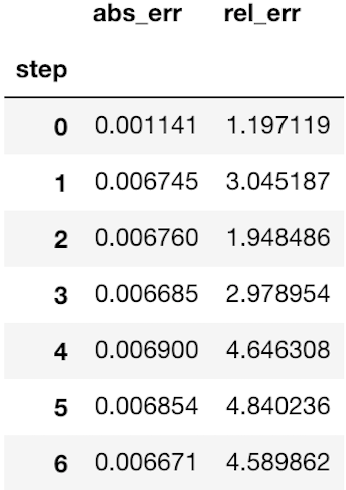
\includegraphics[scale=0.6]{err_step.png}
  \caption{Accuracy in predicting $y_{t+h}$ given $x_t$ }
  \label{err_step}
\end{figure}

and focusing only on the one-step ahead prediction:
\begin{figure}[h!]
  \centering
  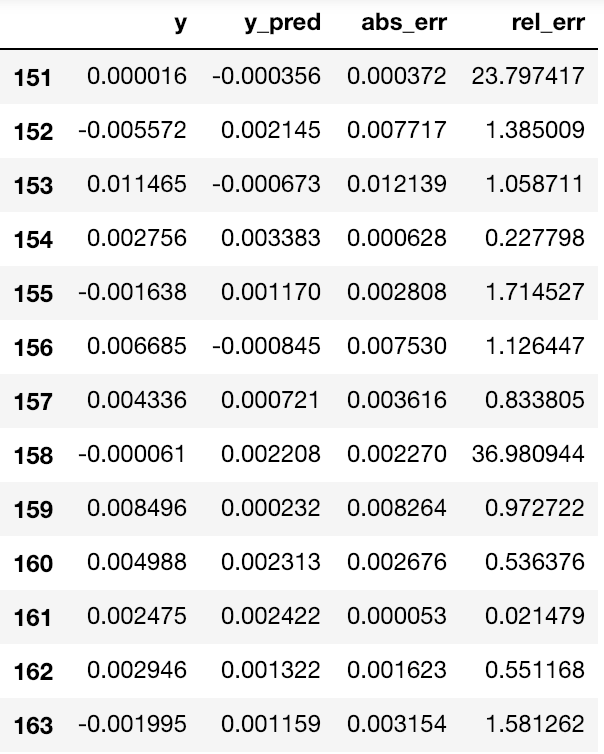
\includegraphics[scale=0.6]{pred_step1.png}
  \caption{One-step ahead prediction}
  \label{err_step}
\end{figure}



\subsection{Parameter estimation}
As we said our principal aim is to replicate the $Sp500$ with a relatively low number of assets. To select the right one we could use, as explained in the previous paragraph, lasso or elastic net regression; now we have to deal with the parameter estimation.

As we said we suppose, as actually happens due to the fact that our index is just a combination of 500 assets, that $Sp500$ has a linear relation with the selected assets. A first and natural choice for the $\beta$ of the model are the one obtained by the non-negative lasso regression or non-negative elastic net regression on the whole set of $Sp500$ constituents. Actually this gives nice results, but we will see in experimental phase that selecting the assets and than estimate the model using non negative OLS works better. 
\\

As stated in the previous paragraph, we will use a moving window approach to build the models for both passive and active portfolio management. It's clear in fact that the size of the used window will affect all the further analysis. After different tests, presented before, we decided to use a window 250 observation long. In this way we end up having enough data to build meaningful models, but not too much, because we want to preserve the time invariance of the data inside the window.





\newpage
\section{Portfolio replication}
In this section we will present the two developed strategies to manage the portfolio. 
One of  the principal aim of portfolio management is the replication of a certain index performance, using only a relatively small number of assets. This is justified by the fact that a portfolio with 50 assets is much more flexible and easy to manage with respect to the one with 500 assets. Also an other good reason is that, depending of the type of taxation, could be necessary to pay a fixed amount of fee for each asset we decide to invest on. So if we are able to find a small subset of the 500 assets able to guarantee similar performances, we will gain in terms of management simplicity and lower taxation.

\subsection{Beta}
Using a moving window of length $250$ and using an appropriate regularization parameter $\lambda$ in order to have a number of variables (i.e number of $\beta$-parameters to estimate), we obtain the following result:
\begin{figure}[h!]
  \centering
  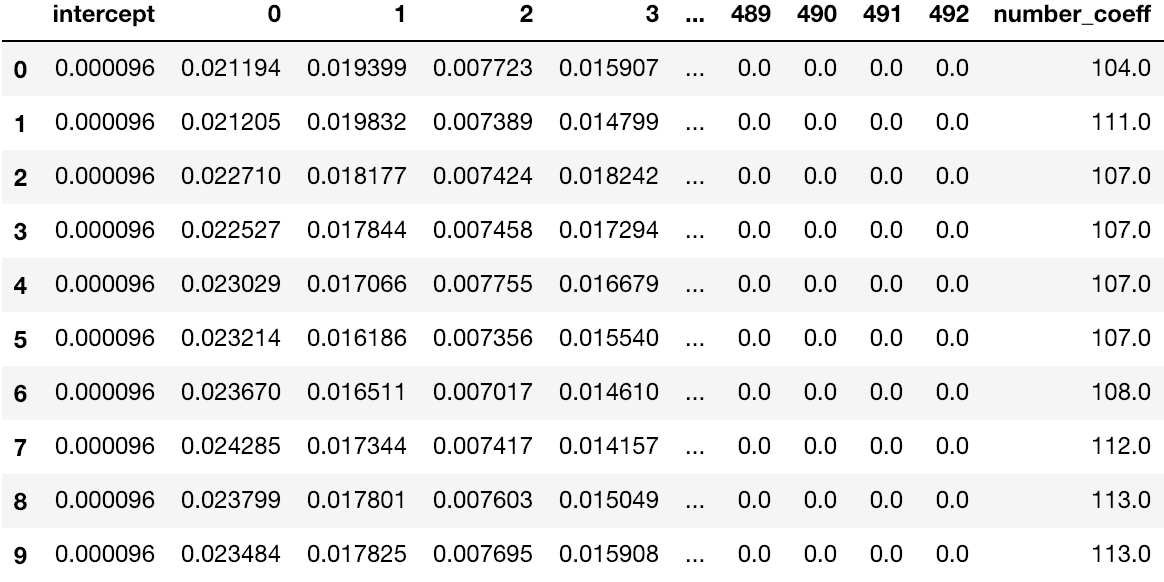
\includegraphics[scale=0.6]{beta_dataset.png}
  \caption{Intercept and $\beta$-coefficients predicted by our model}
  \label{beta_dataset}
\end{figure}
We want to understand how rapidly these $\beta$-parameters change, in particular the turnover among the variables and, in case the model trained in the window$[t+1:t+251]$  introduce a new variable with respect to the model trained in the window$[t:t+250]$, which is the weight of this new variable inside the model (and vice versa for a variable leaving the model). What we get is that on average only $5.49$ new variables are added to the new model (circa $4\%$) and $5.47$ are removed (circa $4\%$). Moreover, new assets enter the model with really low weight (so they still are almost irrelevant) and on the other hand leaving variables are unsurprisingly among the least important in the previous model. In fact, the mean value of the $\beta$-coefficients of the new variables is $0.000858$ (compared with a $0.006668$ mean value of all the $\beta$-coefficients of the chosen variables, only the $0.12\%$ of the chosen variables has a lower weight). We have a similar result also for the variables leaving the model.
\begin{figure}[h!]
  \centering
  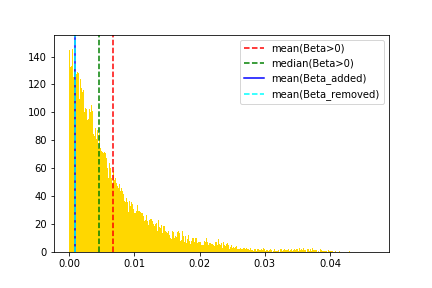
\includegraphics[scale=0.6]{turnover.png}
  \caption{Relevance of the added/removed variables inside the model}
  \label{turnover}
\end{figure}
These results show that we can assume that our "relevant" variables, the ones chosen by our Lasso model at time $t$, will probably still be the important ones at time $t+1$ due to the fact that the only few turnovers we have are among the least important assets.


\subsection{Passive approach}

With passive approach, given that one tries to choose a growing index, we want to mimic as much as possible the index itself, in order to have its same performances.
We will work with $Sp500$, below we report the $Sp500$ time series.


	IMMAGINE     SP500
	
As it's clear by the plot, the considered index, on average, grows with time, so we would have been able to perform just like the index also our portfolio would have increased its value.
\\

In previous paragraphs we already underlined how we could use Lasso in order to select the right subset of asset. So our passive approach to portfolio replication problem will be handled using lasso or elastic net.

A first way to build the portfolio is to use non negative lasso regression on the starting window, representing the time at which one decides to starts to invest, and distribute the budget proportionally to the $\beta_{lasso}$. 










\end{document}